% PREAMBLE
\documentclass[12pt]{article}
\usepackage{amssymb, amsmath, amsthm}
   % libraries of additional mathematics commands  
\usepackage[paper=letterpaper, margin=1in]{geometry}
   % sets margins and space for headers
\usepackage{setspace, listings}
   % allow for adjusted line spacing and printing source code
\usepackage{graphicx}
\graphicspath{ {./images/} }
\title{MATH 310L112\\
       Introduction to Mathematical Reasoning\\
       Assignment \#10}
\author{Michael Wise}
\date{April 26th, 2020}
% END PREAMBLE 

\begin{document}
\maketitle
%\thispagestyle{empty}
\begin{description}
\section*{Section 11.1}
\item[Exercise 4:] Here is a diagram for a relation $R$ on set $A$. Write the sets $A$ and $R$.
\begin{center}
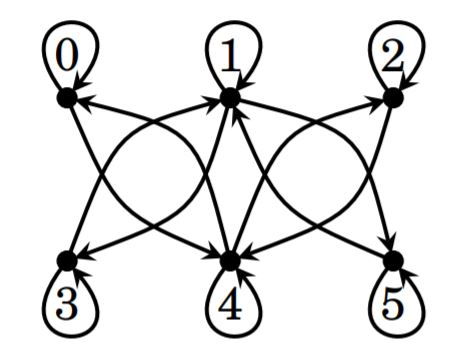
\includegraphics[scale = .4]{images/11.1ex4.JPG}
\end{center}
\begin{spacing}{2}
\begin{proof}[Solution]
The set $A = \{0,1,2,3,4,5\}$. As a set, the relation $R = \{(0,0), (0,4), (1,1), 
\newline
(1,3), (1,5), (2,2), (2,4), (3,3), (3,1), (4,4), (4,0), (4,2), (5,5), (5,1)\}$.
\end{proof}
\end{spacing}
\item[Exercise 10:] Consider the subset $R = (\mathbb{R} \times \mathbb{R}) - \{(x,x):x \in \mathbb{R}\} \subseteq \mathbb{R} \times \mathbb{R}.$ What familiar relation on $\mathbb{R}$ is this? Explain.
\begin{spacing}{2}
\begin{proof}[Solution]
In this example, we have removed all ordered pairs where the coordinates are the same. The relation can also be written as $R = \{(x,y) \in \mathbb{R} \times \mathbb{R}: x \neq y\}$. Thus, $x R y$ if and only if $x \neq y$.
\end{proof}
\end{spacing} 
\section*{Section 11.2}
\item[Exercise 4:] Let $A = \{a,b,c,d\}$. Suppose $R$ is the relation
\begin{align*}
    R = \{(a,a),(b,b),(c,c),(d,d),(a,b),(b,a),(a,c),(c,a), \\
(a,d),(d,a),(b, c),(c,b),(b,d),(d,b),(c,d),(d, c)\}.
\end{align*}
Is $R$ reflexive? Symmetric? Transitive? If a property does not hold, say why.
\begin{spacing}{2}
\begin{proof}[Solution]
Observe that $R$ is \textbf{reflexive} because $(a,a),(b,b),(c,c),(d,d) \in R$. It also clearly follows that $R$ is \textbf{symmetric} because  $xRy$ implies $yRx$ for all $x,y \in A$. (i.e. $(a,b) \in R \Rightarrow (b,a) \in R$, and so on). Finally, observe that $R$ is \textbf{transitive} because whenever $xRy$ and $yRz$, then also $xRz$ for every $x,y,z \in A$. (i.e. $(a,b),(b,c) \in R \Rightarrow (a,c) \in R$).
\end{proof}
\end{spacing} 
\item[Exercise 16:] Define a relation $R$ on $\mathbb{Z}$ by declaring that $xRy$ if and only if $x^2 \equiv y^2 \pmod{4}$. Prove that $R$ is reflexive, symmetric, and transitive.
\begin{spacing}{2}
\begin{proof}
Consider the set $R = \{(x,y) \in \mathbb{Z} \times \mathbb{Z}: x^2 \equiv y^2 \pmod{4}\}$.
\newline
First we will show that $R$ is reflexive. Take any integer $x \in \mathbb{Z}$. Observe that $4 \mid 0$, and therefore $4 \mid (x^2 - x^2)$. By definition, we have that $x^2 \equiv x^2 \pmod{4}$. Thus, $xRx$ for every $x \in \mathbb{Z}$, which shows $R$ is reflexive.
\newline
Next, we will show that $R$ is symmetric. We must show that for all $x,y \in \mathbb{Z}$, the condition $x^2 \equiv y^2 \pmod{4}$ implies $y^2 \equiv x^2 \pmod{4}$. We use direct proof. Let $x,y \in \mathbb{Z}$ so that $xRy$. This means $x^2 \equiv y^2 \pmod{4}$. By definition, $4 \mid (x^2 - y^2)$. Then $x^2-y^2 = 4k$ for some $k \in \mathbb{Z}$. Multiplying both sides by $-1$ gives us $y^2 - x^2 = 4(-k)$. Therefore $4 \mid (y^2 - x^2)$ and $y^2 \equiv x^2 \pmod{4}$. Since $xRy$ implies $yRx$ we have shown that $R$ is symmetric.
\newline
Finally we show that $R$ is transitive.  We must show that if $x^2 \equiv y^2 \pmod{4}$ and $y^2 \equiv z^2 \pmod{4}$, then $x^2 \equiv z^2 \pmod{4}$. We use direct proof once more. Suppose that $x^2 \equiv y^2 \pmod{4}$ and $y^2 \equiv z^2 \pmod{4}$. This means $4 \mid (x^2-y^2)$ and $4 \mid (y^2-z^2)$. Then $x^2-y^2 = 4k$ and $y^2 - z^2 = 4l$ for some $k,l \in \mathbb{Z}$ by definition. Adding the two equations gets us $x^2 - z^2 = 4k + 4l$. Therefore, $x^2 - z^2 = 4(k+l)$, so $4 \mid (x^2 - z^2)$, thus $x^2 \equiv z^2 \pmod{4}$. We have just shown $R$ is transitive.
\newline
Since the relation $R$ is reflexive, symmetric, and transitive, we are done.
\end{proof}
\end{spacing} 
\section*{Section 11.3}
\item[Exercise 8:] Define a relation $R$ on $\mathbb{Z}$ as $xRy$ if and only if $x^2+y^2$ is even. Prove $R$ is an equivalence relation. Describe its equivalence classes.
\begin{spacing}{2}
\begin{proof}
In order to show that $R$ is an equivalence relation, we must prove that $R$ is reflexive, symmetric, and transitive.
\newline
We begin by showing that $R$ is reflexive. Let $x \in \mathbb{Z}$ such that $xRx$. Therefore we have $x^2 + x^2 = 2x^2$. Since $x^2 \in \mathbb{Z}$, the quantity $x^2 + x^2$ is even. Thus $xRx$ which means that $R$ is reflexive.
\newline
To show that $R$ is symmetric, let $x,y \in \mathbb{Z}$ such that $xRy$. Obviously $x^2 + y^2 = y^2 + x^2$ is even by the commutative property. Because $xRy$ implies $yRx$, it follows that $R$ is symmetric.
\newline
Lastly, we show that $R$ is transitive. Let $x,y,z \in \mathbb{Z}$ such that $xRy$ and $yRz$. Then $x^2 + y^2$ is even and $y^2 + z^2$ is even. By definition, $x^2 + y^2 = 2k$ and $y^2 + z^2 = 2l$ for some $k,l \in \mathbb{Z}$. Therefore $x^2 = 2k - y^2$ and $z^2 = 2l - y^2$. Adding the equations together gives us
\begin{align*}
    x^2 + z^2 &= 2k + 2l - 2y^2 \\
    &= 2(k + l - y^2).
\end{align*}
Since $k + l - y^2$ is an integer, $x^2 + z^2$ is even by definition. Hence, $xRz$, which proves that $R$ is transitive. Thus, the relation $R$ is an equivalence relation.
\end{proof}
Observe how that for the sum of two numbers to be even, they both must have the same parity. Consequently, for $x \in \mathbb{Z}$, we know $x^2$ is even if and only if $x$ is even (which also holds true for odd integers). Thus we have two equivalence classes:
\begin{align*}
    [0] &= \{x \in \mathbb{Z} : x^2 \text{ is even}\} \\
    [1] &= \{x \in \mathbb{Z} : x^2 \text{ is odd}\}
\end{align*}
where $[0] = [2] = [4] = \cdots$ and $[1] = [3] = [5] = \cdots$ similarly.
\end{spacing}
\item[Exercise 12:] Prove or disprove: If $R$ and $S$ are two equivalence relations on a set $A$, then $R \cup S$ is also an equivalence relation on $A$.
\begin{spacing}{2}
\begin{proof}[Disproof]
This statement is \textbf{false} because of the following counterexample.
\newline
Let $A = \{1,2,3\}$. Now suppose $R$ is a relation on $A$ defined by $R = \{(1,1),(2,2),
\newline 
(3,3),(1,2),(2,1)\}$. Let $S$ be a relation on $A$ defined by $S = \{(1,1),(2,2), (3,3),
\newline
(1,3),(3,1)\}$. Both $R$ and $S$ are equivalence relations on $A$ because they are reflexive, symmetric, and transitive. However, consider $R \cup S$:
\begin{align*}
    R \cup S = \{(1,1),(2,2),(3,3),(1,2),(2,1),(1,3),(3,1)\}.
\end{align*}
Observe how $R \cup S$ contains $(2,1)$ and $(1,3)$, but not $(2,3)$. Because $R \cup S$ is not transitive, then it is not an equivalence relation on $A$. Thus, the statement is false.
\end{proof}
\end{spacing} 
\section*{Section 11.4}
\item[Exercise 2:] List all the partitions of the set $A = \{a,b,c\}$. Compare your answer to the answer to Exercise 6 of Section 11.3.
\begin{spacing}{2}
\begin{proof}[Solution]
Let the set $A = \{a,b,c\}$. The partitions of set $A$ are:
\begin{align*}
    &\Big\{\{a\},\{b\},\{c\}\Big\}, \\
    &\Big\{\{a,b\},\{c\}\Big\}, \\
    &\Big\{\{b,c\},\{a\}\Big\}, \\
    &\Big\{\{a,c\},\{b\}\Big\}, \\
    &\Big\{\{a,b,c\}\Big\}.
\end{align*}
The 5 partitions of $A$ correspond to the 5 equivalence relations of $A$ that are found in Exercise 6 of Section 11.3.
\end{proof}
\end{spacing} 
\end{description}
%%%%%%%%%%%%%%%%%%%%%%%%%%%%%%%%%%%%%%%%%%%%%%%%%%%%%%%%%%%%%%
% The commands in this section print the source code starting
% on a new page. Comment out or delete if you do not want to 
% include the source code in your document.
%
\newpage
\lstset{
   basicstyle=\footnotesize\ttfamily,
   breaklines=true,
   language=[LaTeX]{TeX}
   }
\lstinputlisting{Assignment10.tex} % Change to correct filename
%
%%%%%%%%%%%%%%%%%%%%%%%%%%%%%%%%%%%%%%%%%%%%%%%%%%%%%%%%%%%%%%
\end{document}